\begin{minipage}{0.4\textwidth}
{\bf Внешняя задача Дирихле}
% Затехал: Цветкова Ольга
Найти $u(x) \in C^2(\Omega) \cap C(\Omega \cup \text{Г})$, удовлетворяющую условиям:
\[
\begin{cases}
\Delta u(x) = 0, \forall x \in \Omega \\
u|_\text{Г} = u_0(x),\ x \in \text{Г} \\
u(x) \rightarrow_{|x|\rightarrow \infty} 0
\end{cases}
\]

Такое решение называется {\bf классическим}

\end{minipage}
\hfill
\begin{minipage}{0.4\textwidth}
{\bf Внешнаяя задача Неймана}

Найти $u(x) \in C^2(\Omega) \cap C(\Omega \cup \text{Г})$, удовлетворяющую условиям:
\[
\begin{cases}
\Delta u(x) = 0, \forall x \in \Omega \\
\cfrac{\partial v}{\partial \bar{\vec n}}|_{\text{Г}} = u_1(x),\ x \in \text{Г} \\
u(x) \rightarrow_{|x|\rightarrow \infty} 0
\end{cases}
\]

Такое решение называется {\bf классическим}

\end{minipage}




Отличие постановок внешних и внутренних задач - $u(x) \rightarrow 0$ во внешних задачах. Для внутренней задачи Неймана - даже при выполнении условий разрешимости $\oint u_1(x) dS_x = 0$ решение не единственно

\begin{theorem}
Не может существовать более 1 классического решения внешней задачи Дирихле
\end{theorem}
\begin{proof}
Если $u_1,\  u_2$ - классические решения, то $v(x) = u_1 - u_2$ -удовлетворяет полностью однородной задаче 
\[
\begin{cases}
v(x)|_{\text{Г}} = 0\\
v(x) \rightarrow_{|x|\rightarrow \infty} 0 \ (\forall \eps > 0 \exists \widetilde{R}(\eps) : \forall x : |x| > \widetilde{R}(\eps) \rightarrow |v(x)|<\eps)
\end{cases}
\]

\begin{center}
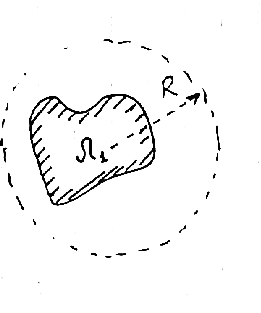
\includegraphics[scale = 0.4]{23_1_new}
\end{center}

Строим сферу радиуса $R \geqslant \widetilde{R}(\eps), \Omega_1 \subset B_R(o)$.
По следствию из принципа максимума $|v(x)|\leqslant~\max\limits_{\partial\Omega_1 \cup \partial B_R(0)} |v(y)|\leqslant ~\eps$

Т.к. $\eps > 0$ было выбрано произвольно, имеем $v(x) \equiv 0 \text{ в } \Omega \cup \text{Г}$
\end{proof}

\begin{theorem}
Не может существовать более 1 классического решения внешней задачи Неймана
\end{theorem}
\begin{proof}
Если $u_1,\  u_2$ - классические решения, то $\underbrace{v(x) = u_1 - u_2}_{\text{гармоническая в }\Omega\text{ и }C^2(\Omega)\cap C^2(\Omega \cup \text{Г})}$ -удовлетворяет полностью однородной задаче 
\[
\begin{cases}
\cfrac{\partial v}{\partial \bar{\vec n}}|_{\text{Г}} = 0\\
v(x) \rightarrow_{|x|\rightarrow \infty} 0 \ (\forall \eps > 0 \exists \widetilde{R}(\eps) : \forall x : |x| > \widetilde{R}(\eps) \rightarrow |v(x)|<\eps)
\end{cases}
\]
\begin{center}
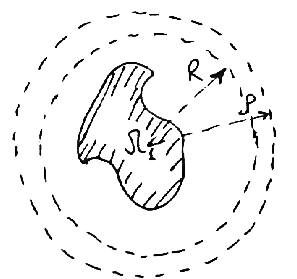
\includegraphics[scale = 0.4]{23_2_new}
\end{center}

Возьмем $R:\ \Omega_1 \subset B_R(0),\ \rho > R$. По I-ф-лу Грина для v
\[
\cancelto{0}{\int\limits_{B_R(0) \backslash \Omega_1} \Delta v \cdot v \cdot dx} = 
\cancelto{0}{\oint\limits_{\text{Г}} \cfrac{\partial v}{\partial \bar{\vec n}} v(x) dS_x} + \oint\limits_{\partial B_R(0)} \cfrac{\partial v}{\partial \bar{\vec n}} v(x) dS_x - \int\limits_{B_R(0) \backslash \Omega_1} |\nabla v(x)|^2 dx
\]

Получили $\int\limits_{B_R(0) \backslash \Omega_1} |\nabla v(x)|^2 dx = \oint\limits_{\partial B_R(0)} \cfrac{\partial v}{\partial \bar{\vec n}} v(x) dS_x$. Далее $\int\limits_{B_R(0) \backslash \Omega_1} |\nabla v(x)|^2 dx \leqslant \int\limits_{B_\rho(0) \backslash \Omega_1} |\nabla v(x)|^2 dx = \oint\limits_{\partial B_\rho(0)} \bigl|\cfrac{\partial v}{\partial \bar{\vec n}}\bigr| |v(x)| dS_x \leqslant (\text{ теорема об асимптотике гармонических функций }) \leqslant \cfrac{C_1}{\rho^2}\cdot \cfrac{C_2}{\rho}\cdot 4\pi\rho^2 \rightarrow 0 \text{ при }\rho \rightarrow \infty$.

Итак, $\nabla v(x) \equiv 0 \Rightarrow v(x) \equiv const = 0$, ч.т.д.
\end{proof}